%=======================+=========================
%================  Reconstruction  ================
%=================================================


\section[Event reconstruction (Alex A.)]{Event reconstruction \label{sec:reconstruction}}

% Copy from GlueX-doc-3108
% "Production and Analysis of GlueX Data"
% TODO: UPDATE for 2017

During and after experimental running, GlueX uses the computer center batch farm to perform data monitoring, event reconstruction, and physics analyses.  For data monitoring, we study the detector hit occupancies, calibration and reconstruction quality, and experimental yields and resolutions for several physics channels.  We monitor a subset of the data as soon as it hits the tape, submitting batch farm jobs via cron job.  Every few weeks, we perform monitoring launches on a subset of the data to study improvements from ongoing calibrations and reconstruction software improvements.  The histograms produced by these monitoring jobs are published to the web, with the ROOT files available for download, so that collaborators can easily study the quality of the data. 

Every few months we perform a major reconstruction launch over all of the data, linking the hits in the various detector systems to reconstruct particles in the physics events.  Monitoring plots from these launches are also published to the web. Finally, about once a month we perform an analysis launch, where we run a collection of user-submitted analysis plugins over the reconstructed data, producing ROOT TTrees for further physics analysis. For all of these launches, we run JANA multithreaded to make efficient use of the available computing resources. %Figure~\ref{fig:offline_monitorA} shows the multithreaded scaling from our monitoring launches is near the theoretical limit.  SWIF is used to manage the batch farm jobs, and is queried to study the performance of the launches.  Figure~\ref{fig:farm-time} shows how many batch farm jobs were in each processing state as function of time our latest reconstruction launch.
The file outputs from these launches are written to the write-through cache, where they are pinned for further use and backed up to tape.  

Production of GlueX data is carried out in a series steps which we will describe for our engineering run. The Spring 2016 Engineering run consisted of about 2000 separate runs (unique run number) with a total data footprint of about $0.5$ PetaBytes. These data were collected in $20$ GigaByte files, with all physics quality runs consisting of multiple files (typically $100$ or more). Of the $2000$ runs, only 236 of those 
were physics runs. The remaining were short runs which were related to engineering and commissioning tests of the experiment. Figure~\ref{fig:production_overview} shows an overview of the different production runs over GlueX data. 

\begin{figure}[h!]\centering
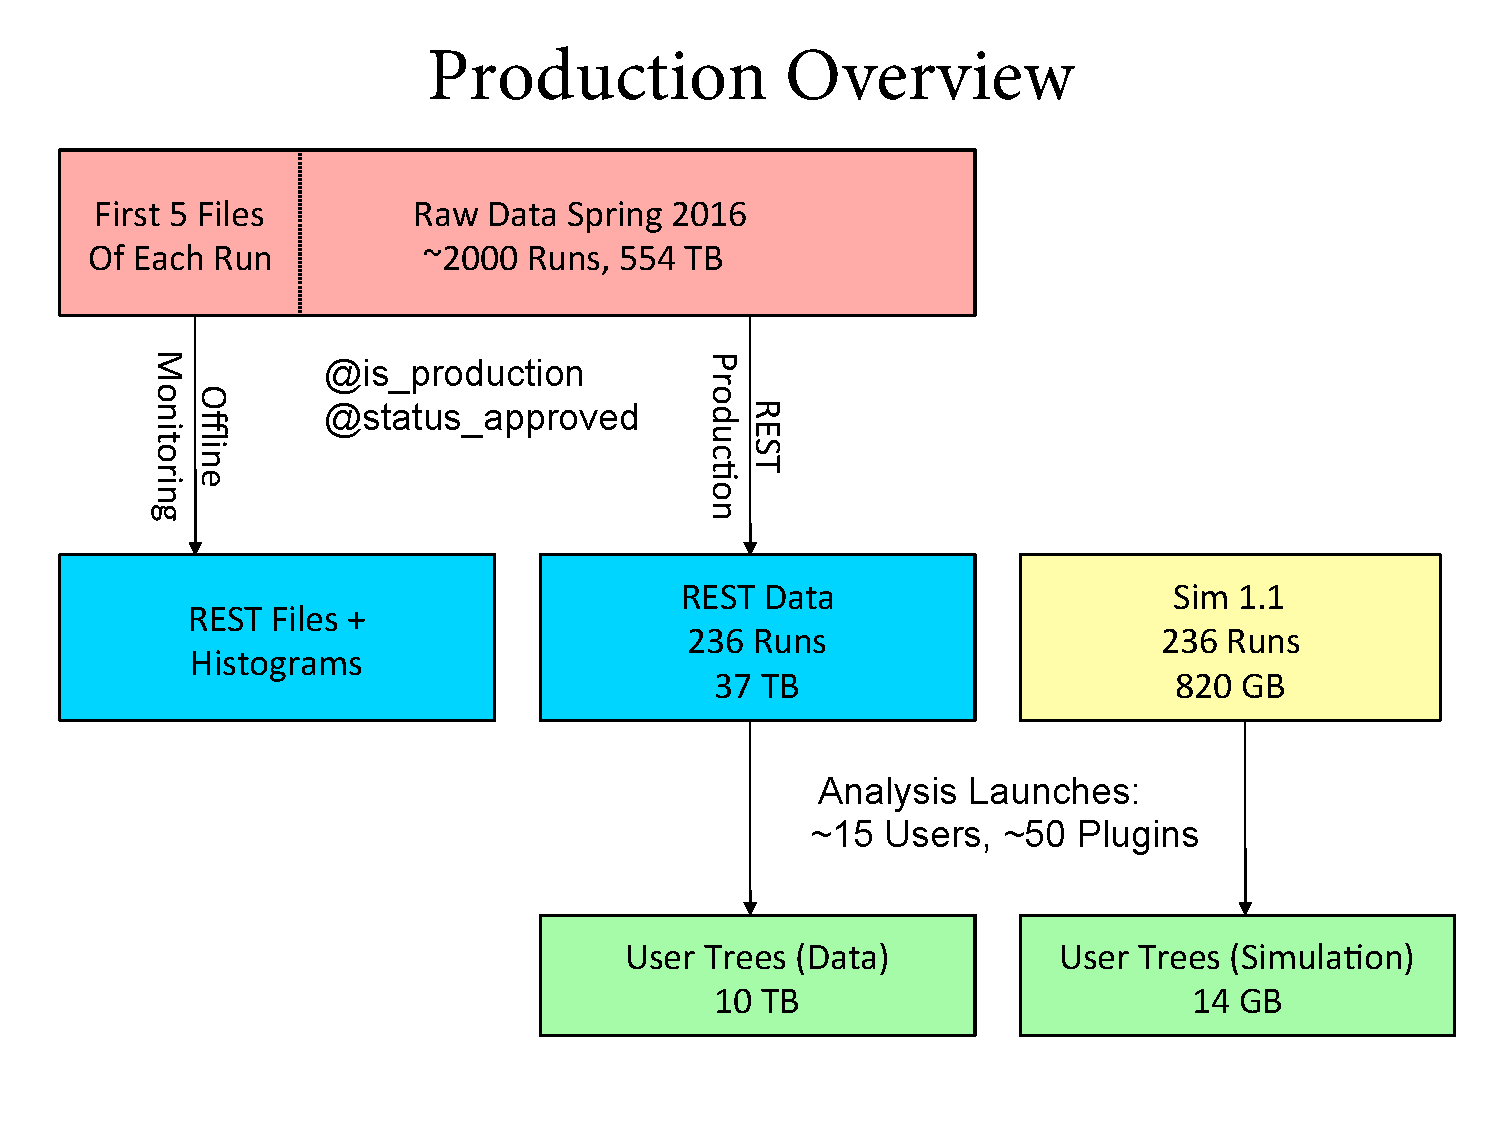
\includegraphics[width=0.8\textwidth]{figures/Production_Spring_2016.pdf}
\caption[]{\label{fig:production_overview}Production flow chart for GlueX data for the Spring 2016 
Engineering run.} 
\end{figure}

\subsection{Calibration pass \label{sec:reccalibration}}

Two types of calibration jobs are running, depending on the complexity of the calibration procedures.  Simple, well-understood calibrations such as timing alignment between individual channels and subdetectors or drift chamber gain and time-to-distance calibrations, can be performed with one file of data per run.  These procedures are run either in the online environment or on the batch farm, and can be run several times as needed due to improvements in reconstruction algorithms or other calibrations.

More complicated calibration procedures, such as calorimeter gain calibration, require more data and are often iterative procedures, requiring several passes through the available data.  The raw data is processed on the batch farm as it comes into the computer center to produce the outputs needed for these procedures, either in the form of histograms or reduced skims in EVIO or ROOT tree format.  Many of these output require that charged particle tracks be reconstructed, but because of the computationally intensive nature of track reconstruction at GlueX, the available computing resources at JLab are insufficient for fully reconstructing all of the raw data as it comes in.  Therefore, only about $10-20$\% of the data has the full suite of calibration procedures applied.  The rest has a limited set of procedures, mostly focused on separating out events collected by specialized triggers. 
The individuals responsible for specific detector calibrations are then responsible for analyzing the skimmed data.

\subsection{Monitoring pass \label{sec:recmonitoring}}

The red-colored box at the top
represents the experimental data that has been copied to the computer center. The small part of the box represents the first five files of each run, which are run through the offline monitoring processes, see section~\ref{sec:onlinemonitoring}. These monitoring jobs are first run during the run to check the quality of the data, but are also run after major changes to calibrations or software to validate those changes. These jobs produce both Reconstructed Events Storage (REST) files and root histogram files for checking job performance.

\subsection{Reconstruction pass \label{sec:recreconstruction}}

We also carry out full production of physics quality data. In the engineering data set, 236 of the
runs were deemed physics quality. We note that while this number is small compared to the total number of runs, it is the vast majority of all data recorded during the running period, 
representing about $400$ TeraBytes of data. All of these files are reconstructed and produce $37$ TeraBytes of REST data files. The large reduction is size from collected event data to physics data files allows us to  more quickly and efficiently carry out physics analyses on the data, and is also small enough to be fully exported to off-site computer centers, see section~\ref{sec:remote-dist}.

In the REST production, we included a series of detector performance studies that required access to raw data and would not be possible on the reconstructed data alone. Many improvements to software and detector calibration resulted from these studies. Similar studies can be made with simulated data to match and assess the detector acceptance.


\subsection{Analysis pass \label{sec:recanalysis}}

The reconstructed (REST) data is also skimmed to produce working data sets for physics. This is described in section~\ref{sec:analysis_skims} and is represented by the left-hand
green box at the bottom of Figure~\ref{fig:production_overview}. Users submit skim code as an \emph{analysis plugin} and it is connected to the master skim job that runs at Jefferson Lab. The skim job shown here had $50$ of these plug-ins and produced about $10$ Terabytes of root files for detailed physics analysis. The volume of these root files is dependent on the number of plug-ins.
